\documentclass{article}
\usepackage[a4paper,
    left=1.8cm,
    right=1.8cm,
    top=2.2cm,
    bottom=2.2cm]{geometry}
\usepackage{longtable}
\usepackage{booktabs}
\usepackage{amsmath}
\usepackage{graphicx}
\usepackage{float} % Required for [H] positioning
\usepackage{tabularx}
\begin{document}
\setlength{\tabcolsep}{3pt}
\begin{table}[H]
\centering
\renewcommand{\arraystretch}{1.3}
\begin{tabularx}{\textwidth}{|p{4cm}|X|}
\hline
\textbf{Experiment No.} & 3 \\ \hline
\textbf{Experiment Title} & Loan Amount Prediction \\ \hline
\textbf{Student Name} & Sathiya Priyan \\ \hline
\textbf{Register Number} & 3122247001058 \\ \hline
\textbf{Faculty} & Dr. Poreddy Ajay Kumar Reddy \\ \hline
\textbf{Submission Date} & 26-07-2026 \\ \hline
\end{tabularx}
\end{table}
\section{Objective} 
The objectives of this experiment are: 
\section{Objective}

The objective of this experiment is to preprocess the Loan Amount Prediction dataset by handling missing values, encoding categorical features, and standardizing the input data for machine learning. The experiment aims to implement and compare Linear Regression, Ridge Regression, Lasso Regression, and Elastic Net Regression models for predicting loan amounts. The performance of these regression models is evaluated using Mean Absolute Error (MAE), Mean Squared Error (MSE), Root Mean Squared Error (RMSE), and the coefficient of determination ($R^2$ Score) to identify the most effective model for loan amount prediction.

%%%%%%%%%%%%%%%%%%%%%%%%%%%%%%%%%%%%%%%%%%%%%%%%%%%%%%%%%%%%%%%%%%%%%% 
\section{Problem Statement} 
The objective of this experiment is to predict the loan amount sanctioned for an applicant based on demographic, financial, and credit-related information.

%%%%%%%%%%%%%%%%%%%%%%%%%%%%%%%%%%%%%%%%%%%%%%%%%%%%%%%%%%%%%%%%%%%%%% 
\section{Dataset Description} 
The experiment uses the \textbf{Loan Amount Prediction} dataset. The dataset contains information about loan applicants including demographic details, employment status, income, credit history, and loan-related attributes. The objective is to predict the continuous target variable \textbf{LoanAmount}. 

\begin{table}[H]
\centering
\renewcommand{\arraystretch}{1.25}
\begin{tabular}{|p{4cm}|p{10.5cm}|}
\hline
\textbf{Attribute} & \textbf{Description} \\ \hline

Loan\_ID &
Unique identifier assigned to each loan application.  \\ \hline

Gender &
Gender of the applicant. \\ \hline

Married &
Marital status of the applicant. \\ \hline

Dependents &
Number of dependents. \\ \hline

Education &
Applicant's education level. \\ \hline

Self\_Employed &
Indicates whether the applicant is self-employed. \\ \hline

ApplicantIncome &
Monthly income of the applicant. \\ \hline

CoapplicantIncome &
Monthly income of the co-applicant. \\ \hline

LoanAmount &
Requested loan amount (Target Variable). \\ \hline

Loan\_Amount\_Term &
Loan repayment term (in months). \\ \hline

Credit\_History &
Credit history of the applicant. \\ \hline

Property\_Area &
Residential area of the property (Urban, Semiurban, or Rural). \\ \hline

Loan\_Status &
Loan approval status in the dataset. \\ \hline

\end{tabular}
\caption{Description of Dataset Attributes}
\label{tab:dataset}
\end{table}
\newpage
\noindent \textbf{Dataset Summary} 
\begin{itemize} 
    \item Number of instances: \textbf{614} 
    \item Number of attributes: \textbf{13} 
    \item Prediction type: \textbf{Regression} 
    \item Target variable: \textbf{LoanAmount} 
    \item Input features: Demographic, financial, employment, credit history, and property-related attributes. 
\end{itemize}

%%%%%%%%%%%%%%%%%%%%%%%%%%%%%%%%%%%%%%%%%%%%%%%%%%%%%%%%%%%%%%%%%%%%%% 
\section{Exploratory Data Analysis (EDA)} 
%%%%%%%%%%%%%%%%%%%%%%%%%%%%%%%%%%%%%%%%%%%%%%%%%%%%%%%%%%%%%%%%%%%%%% 
\subsection{Dataset Overview} 
The Loan Amount Prediction dataset contains information about loan applicants, including demographic details, income, employment status, credit history, property area, and loan-related attributes. The dataset consists of both categorical and numerical features. 

The dataset contains: 
\begin{itemize} 
    \item Number of observations: \textbf{614} 
    \item Number of attributes: \textbf{13} 
    \item Numerical features: 5 
    \item Categorical features: 8 
    \item Target variable: \textbf{LoanAmount} 
\end{itemize} 
The dataset includes missing values in several attributes, which are handled during the preprocessing stage. 

%%%%%%%%%%%%%%%%%%%%%%%%%%%%%%%%%%%%%%%%%%%%%%%%%%%%%%%%%%%%%%%%%%%%%% 
\subsection{Statistical Summary} 
The statistical summary provides useful insights into the numerical attributes of the dataset. 

\begin{table}[H] 
\centering 
\caption{Summary Statistics of Numerical Features} 
\begin{tabular}{|l|c|c|c|c|} 
\hline 
\textbf{Feature} & \textbf{Mean} & \textbf{Median} & \textbf{Minimum} & \textbf{Maximum}\\ \hline 
ApplicantIncome & 5403.46 & 3812.50 & 150 & 81000\\ 
CoapplicantIncome & 1621.25 & 1188.50 & 0 & 41667\\ 
LoanAmount & 146.41 & 128.00 & 9 & 700\\ 
Loan\_Amount\_Term & 342.00 & 360.00 & 12 & 480\\ 
Credit\_History & 0.842 & 1.00 & 0 & 1\\ \hline 
\end{tabular} 
\end{table} 

\noindent \textbf{Inference} 
\begin{itemize} 
    \item Applicant income varies significantly among applicants. 
    \item Most applicants have a loan term of 360 months. 
    \item Credit history values are predominantly equal to 1, indicating that most applicants possess a good credit history. 
    \item Loan amounts range from very small values to high-value loans, suggesting the presence of outliers. 
\end{itemize} 

%%%%%%%%%%%%%%%%%%%%%%%%%%%%%%%%%%%%%%%%%%%%%%%%%%%%%%%%%%%%%%%%%%%%%% 
\subsection{Missing Value Analysis} 
Several attributes contain missing values. 

\begin{table}[H] 
\centering 
\caption{Missing Values in Dataset} 
\begin{tabular}{|l|c|} 
\hline 
\textbf{Feature} & \textbf{Missing Values}\\ \hline 
Gender & 13\\ 
Married & 3\\ 
Dependents & 15\\ 
Self\_Employed & 32\\ 
LoanAmount & 22\\ 
Loan\_Amount\_Term & 14\\ 
Credit\_History & 50\\ \hline 
\end{tabular} 
\end{table} 

\noindent \textbf{Inference} 
\begin{itemize} 
    \item Missing values are present in both categorical and numerical attributes. 
    \item Credit\_History contains the highest number of missing values. 
    \item Proper imputation is necessary before model training to avoid information loss. 
\end{itemize} 

%%%%%%%%%%%%%%%%%%%%%%%%%%%%%%%%%%%%%%%%%%%%%%%%%%%%%%%%%%%%%%%%%%%%%% 
\subsection{Distribution of Loan Amount} 
The distribution of the target variable was analyzed using a histogram. 

\begin{figure}[H]
    \centering
    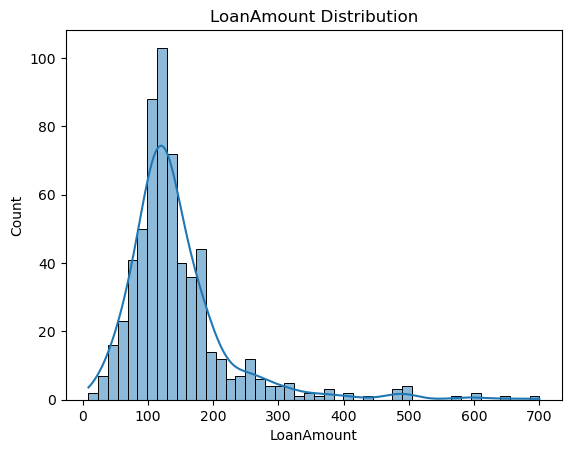
\includegraphics[width=0.75\linewidth]{loan_distribution.png}
    \caption{Distribution of Loan Amount}
    \label{fig:loan_distribution}
\end{figure}

\noindent \textbf{Inference} 
\begin{itemize} 
    \item Loan amounts are not uniformly distributed. 
    \item Most loan applications request comparatively smaller loan amounts. 
    \item A few observations correspond to very large loans, producing a positively skewed distribution. 
\end{itemize} 

%%%%%%%%%%%%%%%%%%%%%%%%%%%%%%%%%%%%%%%%%%%%%%%%%%%%%%%%%%%%%%%%%%%%%% 
\subsection{Correlation Matrix} 
A correlation matrix is useful for identifying relationships among numerical variables. 

\begin{figure}[H] 
\centering 
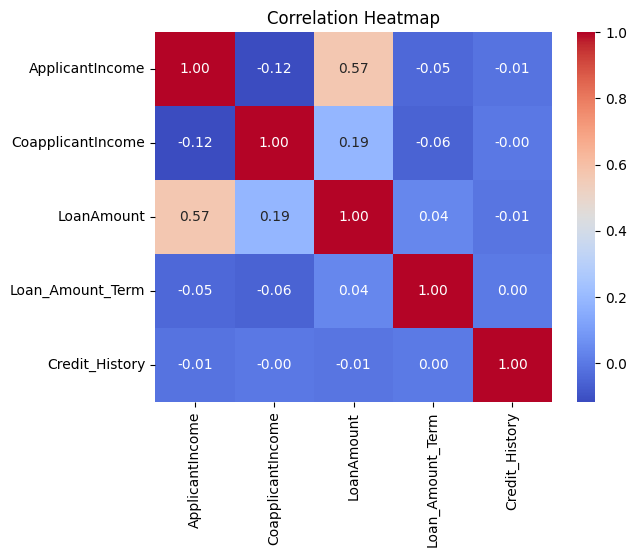
\includegraphics[width=0.85\linewidth]{correlation_matrix.png} 
\caption{Correlation Matrix of Numerical Features} 
\label{fig:corr} 
\end{figure} 

\noindent \textbf{Inference} 
\begin{itemize} 
    \item ApplicantIncome and LoanAmount exhibit a positive relationship. 
    \item CoapplicantIncome also contributes positively toward LoanAmount. 
    \item Credit history has comparatively weak correlation with the regression target. 
    \item No pair of numerical variables shows extremely high correlation, reducing the likelihood of severe multicollinearity. 
\end{itemize} 

%%%%%%%%%%%%%%%%%%%%%%%%%%%%%%%%%%%%%%%%%%%%%%%%%%%%%%%%%%%%%%%%%%%%%% 
\subsection{Overall EDA Observations} 
\begin{itemize} 
    \item The dataset contains 614 loan application records with a mixture of categorical and numerical features. 
    \item Missing values are present and require preprocessing before model training. 
    \item LoanAmount exhibits a positively skewed distribution with a few large-valued observations. 
    \item Applicant income varies considerably across applicants, indicating a diverse financial profile. 
    \item The dataset is suitable for regression after appropriate preprocessing, encoding, and feature scaling. 
\end{itemize}
%%%%%%%%%%%%%%%%%%%%%%%%%%%%%%%%%%%%%%%%%%%%%%%%%%%%%%%%%%%%%%%%%%%%%%
\section{Data Preprocessing}
%%%%%%%%%%%%%%%%%%%%%%%%%%%%%%%%%%%%%%%%%%%%%%%%%%%%%%%%%%%%%%%%%%%%%%

The raw dataset contained missing values and categorical attributes that required preprocessing before model training. The following preprocessing steps were performed:

\begin{enumerate}
    \item The \textbf{Loan\_ID} column was removed since it is only an identifier and does not contribute to prediction.
    
    \item Missing values in categorical attributes such as \textbf{Gender}, \textbf{Married}, \textbf{Dependents}, and \textbf{Self\_Employed} were replaced using the mode of the respective column.
    
    \item Missing values in numerical attributes such as \textbf{Loan\_Amount\_Term} and \textbf{Credit\_History} were replaced using the median value.
    
    \item The target variable (\textbf{LoanAmount}) was separated from the feature set.
    
    \item Categorical attributes were converted into numerical form using One-Hot Encoding with \texttt{drop\_first=True}.
    
    \item The dataset was divided into training and testing sets using an 80:20 ratio.
    
    \item Feature scaling was performed using the StandardScaler to normalize numerical features before training the regression models.
\end{enumerate}

%%%%%%%%%%%%%%%%%%%%%%%%%%%%%%%%%%%%%%%%%%%%%%%%%%%%%%%%%%%%%%%%%%%%%%
\section{Regression Algorithms}
%%%%%%%%%%%%%%%%%%%%%%%%%%%%%%%%%%%%%%%%%%%%%%%%%%%%%%%%%%%%%%%%%%%%%%

\subsection{Linear Regression}

Linear Regression is a supervised machine learning algorithm used to predict a continuous target variable by establishing a linear relationship between the dependent variable and one or more independent variables.

The prediction equation is

\[
\hat{y}=\beta_0+\beta_1x_1+\beta_2x_2+\cdots+\beta_nx_n
\]

where

\begin{itemize}
\item $\hat{y}$ is the predicted loan amount.
\item $\beta_0$ is the intercept.
\item $\beta_i$ are regression coefficients.
\item $x_i$ are the input features.
\end{itemize}

\textbf{Advantages}

\begin{itemize}
\item Simple and easy to interpret.
\item Fast to train.
\item Works well for linear relationships.
\item Provides a good baseline regression model.
\end{itemize}

\textbf{Limitations}

\begin{itemize}
\item Sensitive to outliers.
\item Cannot model nonlinear relationships.
\item May suffer from multicollinearity.
\end{itemize}

%%%%%%%%%%%%%%%%%%%%%%%%%%%%%%%%%%%%%%%%%%%%%%%%%%%%%%%%%%%%%%%%%%%%%%

\subsection{Ridge Regression}

Ridge Regression extends Linear Regression by adding an L2 regularization term to reduce model complexity and prevent overfitting.

The optimization objective is

\[
J(\beta)=
\sum_{i=1}^{n}(y_i-\hat{y_i})^2
+
\lambda
\sum_{j=1}^{p}\beta_j^2
\]

where $\lambda$ is the regularization parameter.

\textbf{Advantages}

\begin{itemize}
\item Reduces overfitting.
\item Handles multicollinearity effectively.
\item Produces more stable coefficient estimates.
\end{itemize}

\textbf{Limitations}

\begin{itemize}
\item Does not eliminate irrelevant features.
\item Requires tuning of the regularization parameter.
\end{itemize}

%%%%%%%%%%%%%%%%%%%%%%%%%%%%%%%%%%%%%%%%%%%%%%%%%%%%%%%%%%%%%%%%%%%%%%

\subsection{Lasso Regression}

Lasso Regression introduces L1 regularization, which can shrink some regression coefficients exactly to zero, thereby performing feature selection.

Its objective function is

\[
J(\beta)=
\sum_{i=1}^{n}(y_i-\hat{y_i})^2
+
\lambda
\sum_{j=1}^{p}|\beta_j|
\]

\textbf{Advantages}

\begin{itemize}
\item Performs automatic feature selection.
\item Produces simpler and more interpretable models.
\item Helps reduce overfitting.
\end{itemize}

\textbf{Limitations}

\begin{itemize}
\item Can remove useful correlated features.
\item Performance depends on selecting an appropriate $\lambda$ value.
\end{itemize}

%%%%%%%%%%%%%%%%%%%%%%%%%%%%%%%%%%%%%%%%%%%%%%%%%%%%%%%%%%%%%%%%%%%%%%

\subsection{Elastic Net Regression}

Elastic Net Regression combines both L1 and L2 regularization to obtain the advantages of Ridge and Lasso Regression.

Its objective function is

\[
J(\beta)=
\sum_{i=1}^{n}(y_i-\hat{y_i})^2
+
\lambda_1
\sum_{j=1}^{p}|\beta_j|
+
\lambda_2
\sum_{j=1}^{p}\beta_j^2
\]

where

\begin{itemize}
\item $\lambda_1$ controls the L1 penalty.
\item $\lambda_2$ controls the L2 penalty.
\end{itemize}

\textbf{Advantages}

\begin{itemize}
\item Combines feature selection and coefficient shrinkage.
\item Performs well with highly correlated features.
\item Reduces overfitting while maintaining prediction accuracy.
\end{itemize}

\textbf{Limitations}

\begin{itemize}
\item More computationally expensive than Linear Regression.
\item Requires tuning of multiple hyperparameters.
\item Interpretation is slightly more complex than Linear Regression.
\end{itemize}

%%%%%%%%%%%%%%%%%%%%%%%%%%%%%%%%%%%%%%%%%%%%%%%%%%%%%%%%%%%%%%%%%%%%%%
\section{Experimental Setup}
%%%%%%%%%%%%%%%%%%%%%%%%%%%%%%%%%%%%%%%%%%%%%%%%%%%%%%%%%%%%%%%%%%%%%%

The experiment was implemented using Python and the Scikit-learn machine learning library. The dataset was divided into training and testing sets using an 80:20 ratio. Numerical features were standardized using the StandardScaler before training the regression models.

The following regression algorithms were implemented:

\begin{itemize}
    \item Linear Regression
    \item Ridge Regression
    \item Lasso Regression
    \item Elastic Net Regression
\end{itemize}

Hyperparameter tuning was performed using GridSearchCV with 5-fold cross-validation to obtain the optimal regularization parameters for Ridge, Lasso, and Elastic Net Regression models.

%%%%%%%%%%%%%%%%%%%%%%%%%%%%%%%%%%%%%%%%%%%%%%%%%%%%%%%%%%%%%%%%%%%%%%
\section{Hyperparameter Tuning using GridSearchCV}
%%%%%%%%%%%%%%%%%%%%%%%%%%%%%%%%%%%%%%%%%%%%%%%%%%%%%%%%%%%%%%%%%%%%%%

GridSearchCV systematically searches over a predefined set of hyperparameters and selects the combination that produces the best cross-validation performance.

\subsection{Ridge Regression}

\begin{table}[H]
\centering
\caption{Best Parameters for Ridge Regression}
\begin{tabular}{|l|c|}
\hline
Parameter & Value\\
\hline
Alpha & 100\\
Cross Validation & 5-fold\\
Best CV $R^2$ Score & 0.2441\\
Training Time (s) & 1.0477\\
\hline
\end{tabular}
\end{table}

%%%%%%%%%%%%%%%%%%%%%%%%%%%%%%%%%%%%%%%%%%%%%%%%%%%%%%%%%%%%%%%%%%%%%%

\subsection{Lasso Regression}

\begin{table}[H]
\centering
\caption{Best Parameters for Lasso Regression}
\begin{tabular}{|l|c|}
\hline
Parameter & Value\\
\hline
Alpha & 0.01\\
Cross Validation & 5-fold\\
Best CV $R^2$ Score & 0.2281\\
Training Time (s) & 0.0243\\
\hline
\end{tabular}
\end{table}

%%%%%%%%%%%%%%%%%%%%%%%%%%%%%%%%%%%%%%%%%%%%%%%%%%%%%%%%%%%%%%%%%%%%%%

\subsection{Elastic Net Regression}

\begin{table}[H]
\centering
\caption{Best Parameters for Elastic Net Regression}
\begin{tabular}{|l|c|}
\hline
Parameter & Value\\
\hline
Alpha & 0.10\\
L1 Ratio & 0.20\\
Cross Validation & 5-fold\\
Best CV $R^2$ Score & 0.2336\\
Training Time (s) & 0.0367\\
\hline
\end{tabular}
\end{table}

%%%%%%%%%%%%%%%%%%%%%%%%%%%%%%%%%%%%%%%%%%%%%%%%%%%%%%%%%%%%%%%%%%%%%%
\section{Performance Evaluation Metrics}
%%%%%%%%%%%%%%%%%%%%%%%%%%%%%%%%%%%%%%%%%%%%%%%%%%%%%%%%%%%%%%%%%%%%%%

The following regression evaluation metrics were used to assess model performance.

\begin{itemize}
    \item Mean Absolute Error (MAE)
    \item Mean Squared Error (MSE)
    \item Root Mean Squared Error (RMSE)
    \item Coefficient of Determination ($R^2$ Score)
\end{itemize}

Lower values of MAE, MSE, and RMSE indicate better prediction accuracy, whereas a higher $R^2$ score indicates better model performance.

%%%%%%%%%%%%%%%%%%%%%%%%%%%%%%%%%%%%%%%%%%%%%%%%%%%%%%%%%%%%%%%%%%%%%%
\section{Experimental Results}
%%%%%%%%%%%%%%%%%%%%%%%%%%%%%%%%%%%%%%%%%%%%%%%%%%%%%%%%%%%%%%%%%%%%%%

\begin{table}[H]
\centering
\caption{Performance Comparison of Regression Models}
\begin{tabular}{|l|c|c|c|c|}
\hline
\textbf{Model} & \textbf{MAE} & \textbf{MSE} & \textbf{RMSE} & \textbf{$R^2$}\\
\hline
Linear Regression & 0.2886 & 0.1676 & 0.4094 & 0.2874\\
Ridge Regression & 0.2923 & 0.1709 & 0.4135 & 0.2732\\
Lasso Regression & 0.2903 & 0.1691 & 0.4112 & 0.2810\\
Elastic Net Regression & 0.2940 & 0.1743 & 0.4175 & 0.2590\\
\hline
\end{tabular}
\end{table}

%%%%%%%%%%%%%%%%%%%%%%%%%%%%%%%%%%%%%%%%%%%%%%%%%%%%%%%%%%%%%%%%%%%%%%
\section{Result Visualization}

\subsection{Loan Amount Distribution}

\begin{figure}[H]
\centering
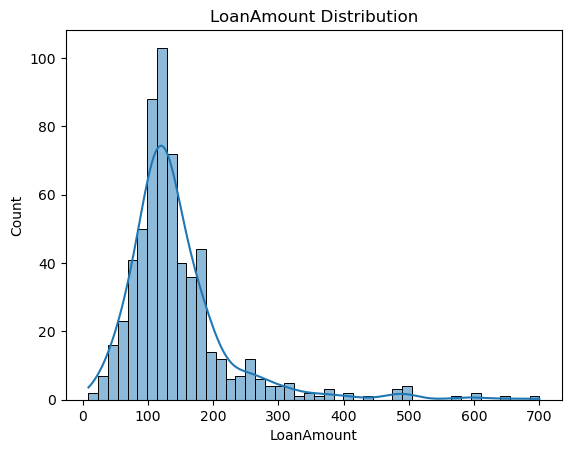
\includegraphics[width=0.7\linewidth]{loan_distribution.png}
\caption{Loan Amount Distribution}
\end{figure}

\textbf{Inference:}
\begin{itemize}
\item The distribution is positively skewed.
\item Most applicants request moderate loan amounts.
\item A few high-value loans appear as outliers.
\end{itemize}

------------------------------------------------

\subsection{Correlation Matrix}

\begin{figure}[H]
\centering
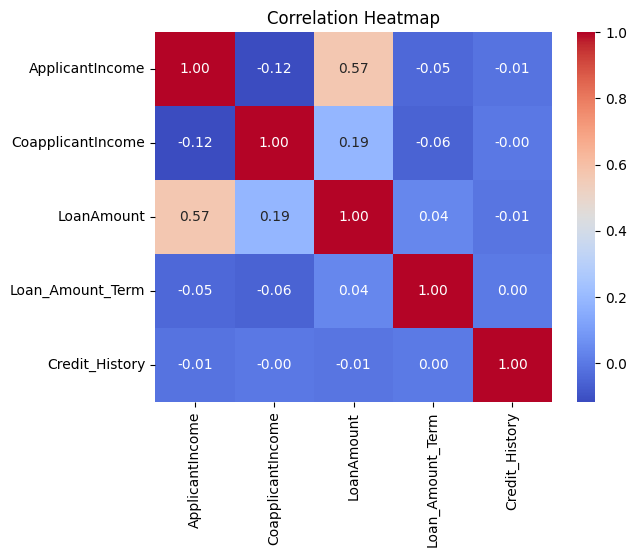
\includegraphics[width=0.8\linewidth]{correlation_matrix.png}
\caption{Correlation Matrix}
\end{figure}

\textbf{Inference:}
\begin{itemize}
\item ApplicantIncome has a positive correlation with LoanAmount.
\item Credit History has a weak correlation with the target variable.
\item No severe multicollinearity is observed.
\end{itemize}

------------------------------------------------

\subsection{Actual vs Predicted}

\begin{figure}[H]
\centering
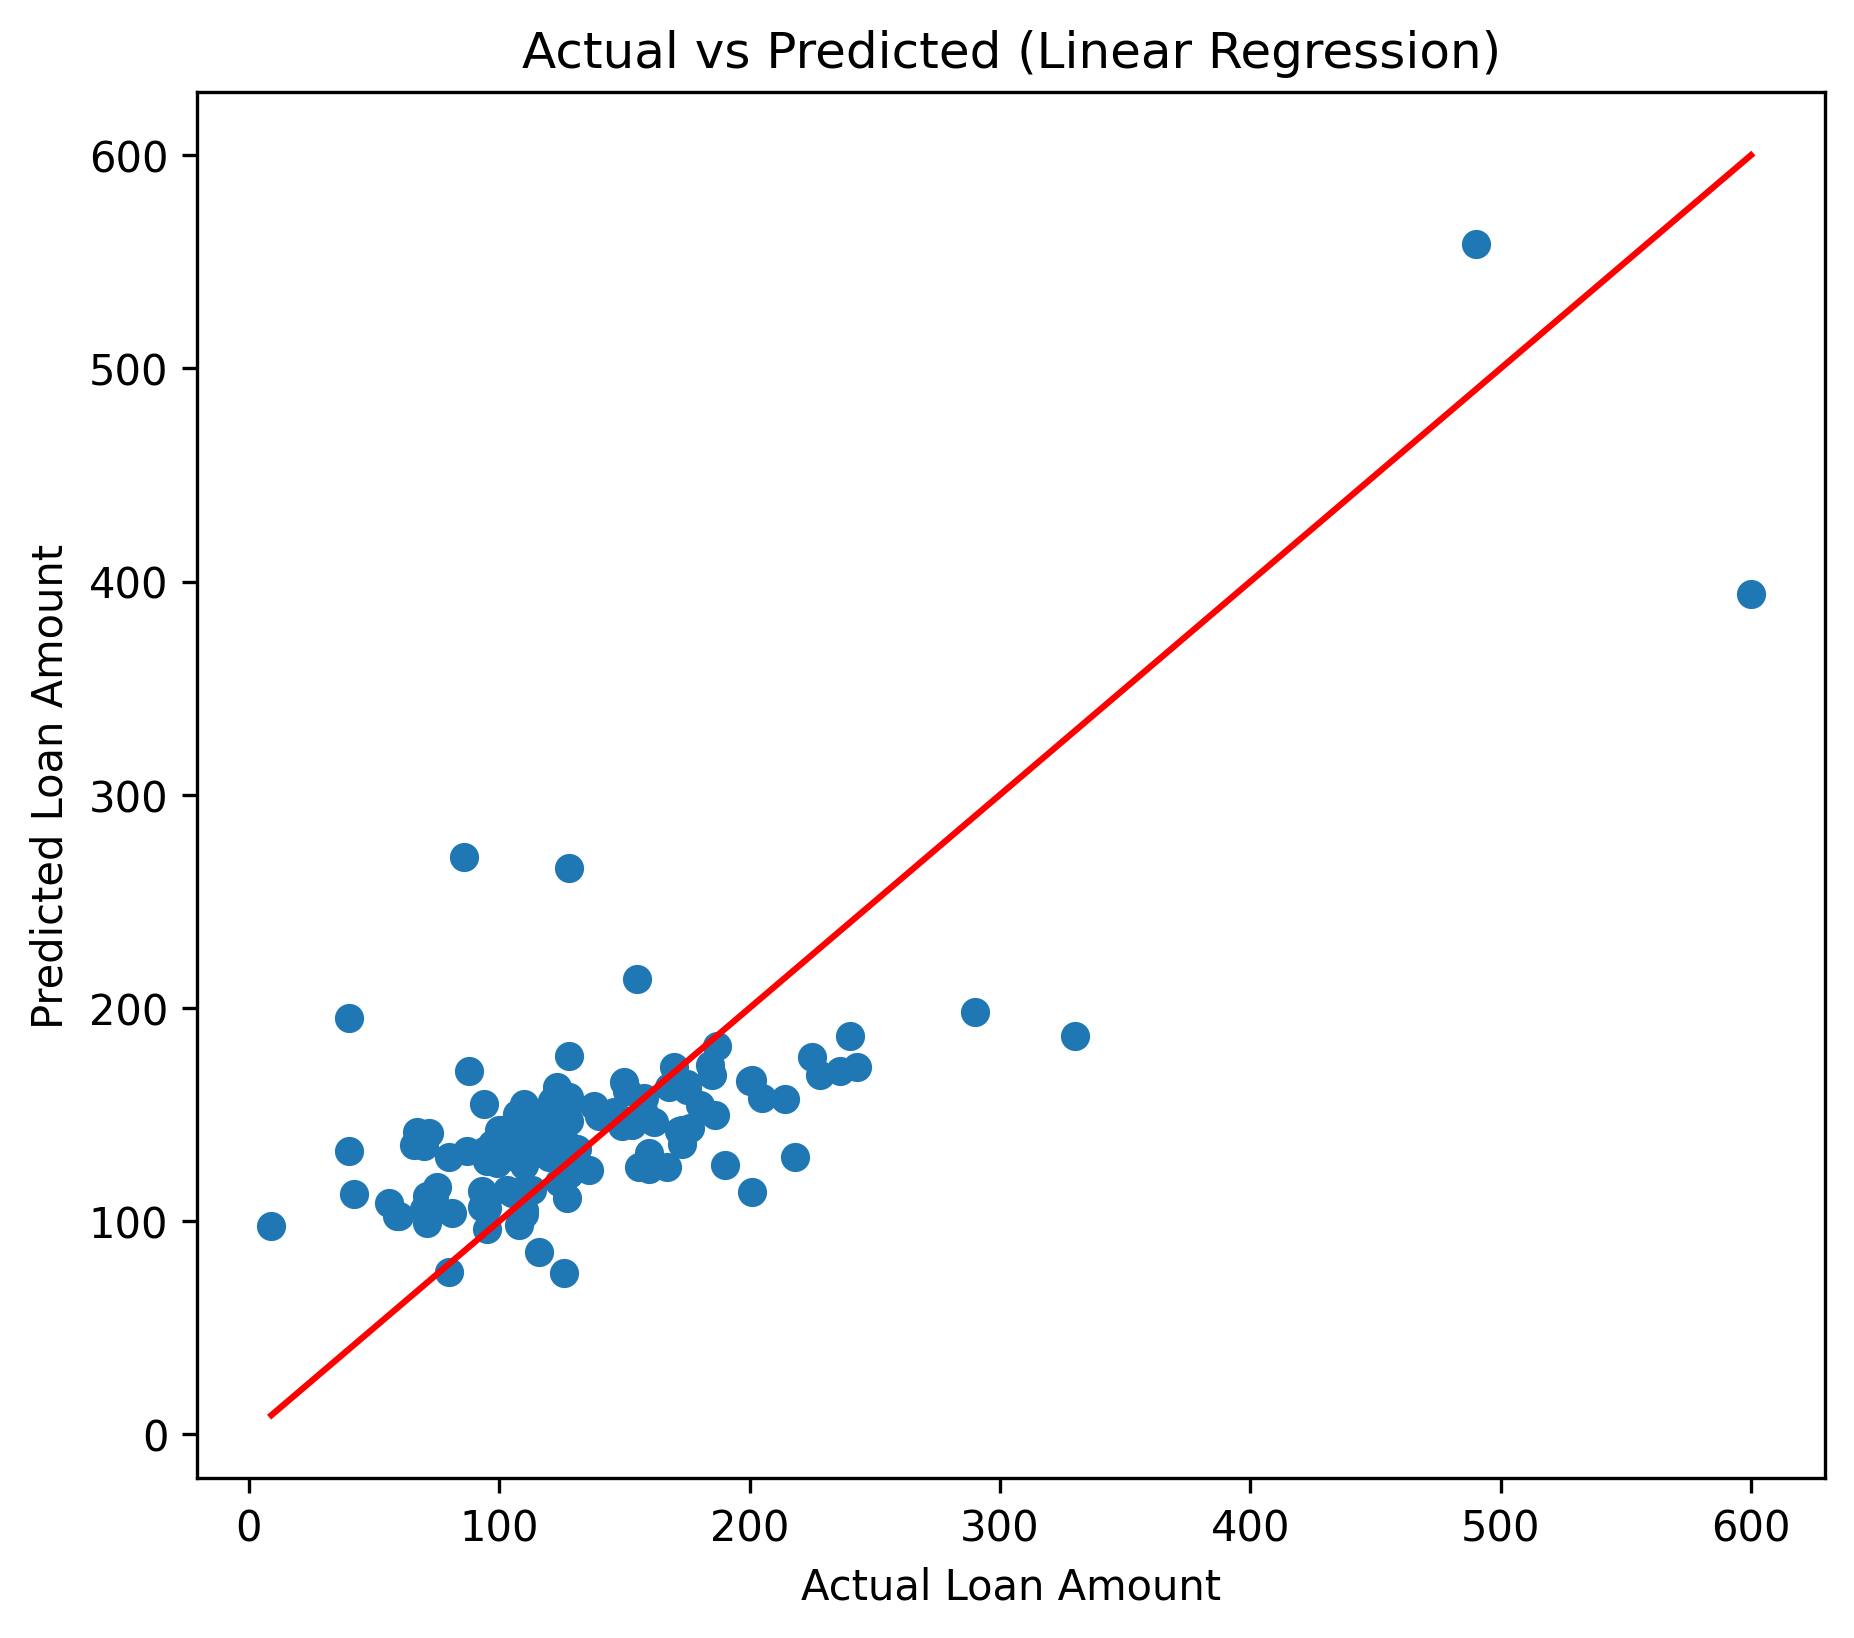
\includegraphics[width=0.7\linewidth]{actual_vs_predicted.png}
\caption{Actual vs Predicted Loan Amount}
\end{figure}

\textbf{Inference:}
\begin{itemize}
\item Most predictions lie close to the ideal diagonal line.
\item The model captures the overall trend reasonably well.
\item Some prediction errors exist for higher loan amounts.
\end{itemize}

------------------------------------------------

\subsection{Residual Plot}

\begin{figure}[H]
\centering
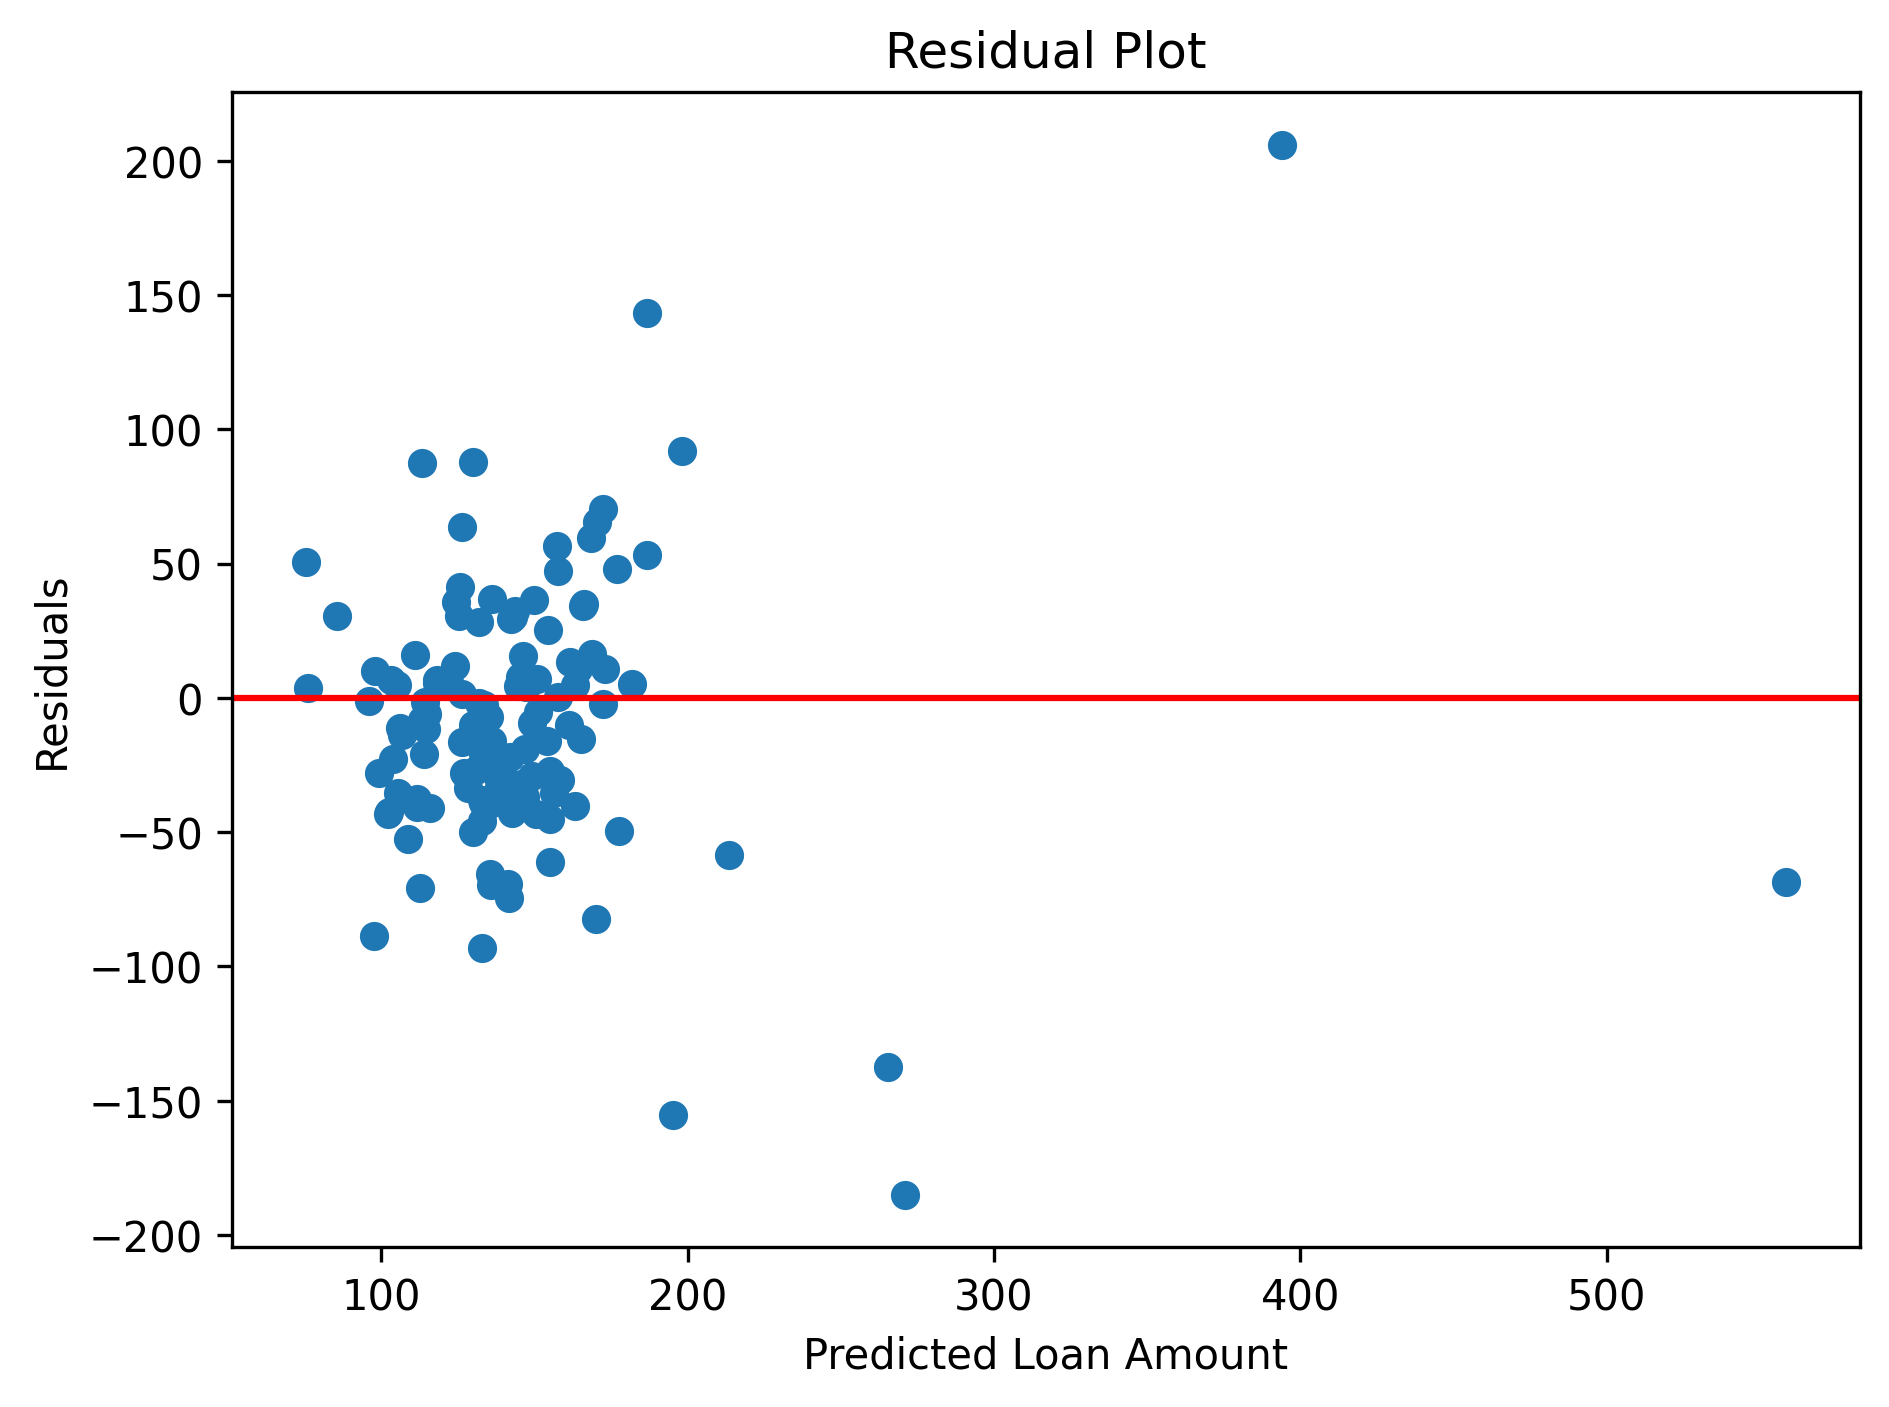
\includegraphics[width=0.7\linewidth]{residual_plot.png}
\caption{Residual Plot}
\end{figure}

\textbf{Inference:}
\begin{itemize}
\item Residuals are randomly distributed around zero.
\item No strong systematic error pattern is observed.
\item The regression model provides an acceptable fit.
\end{itemize}

------------------------------------------------

\subsection{Model Comparison}

\begin{figure}[H]
\centering
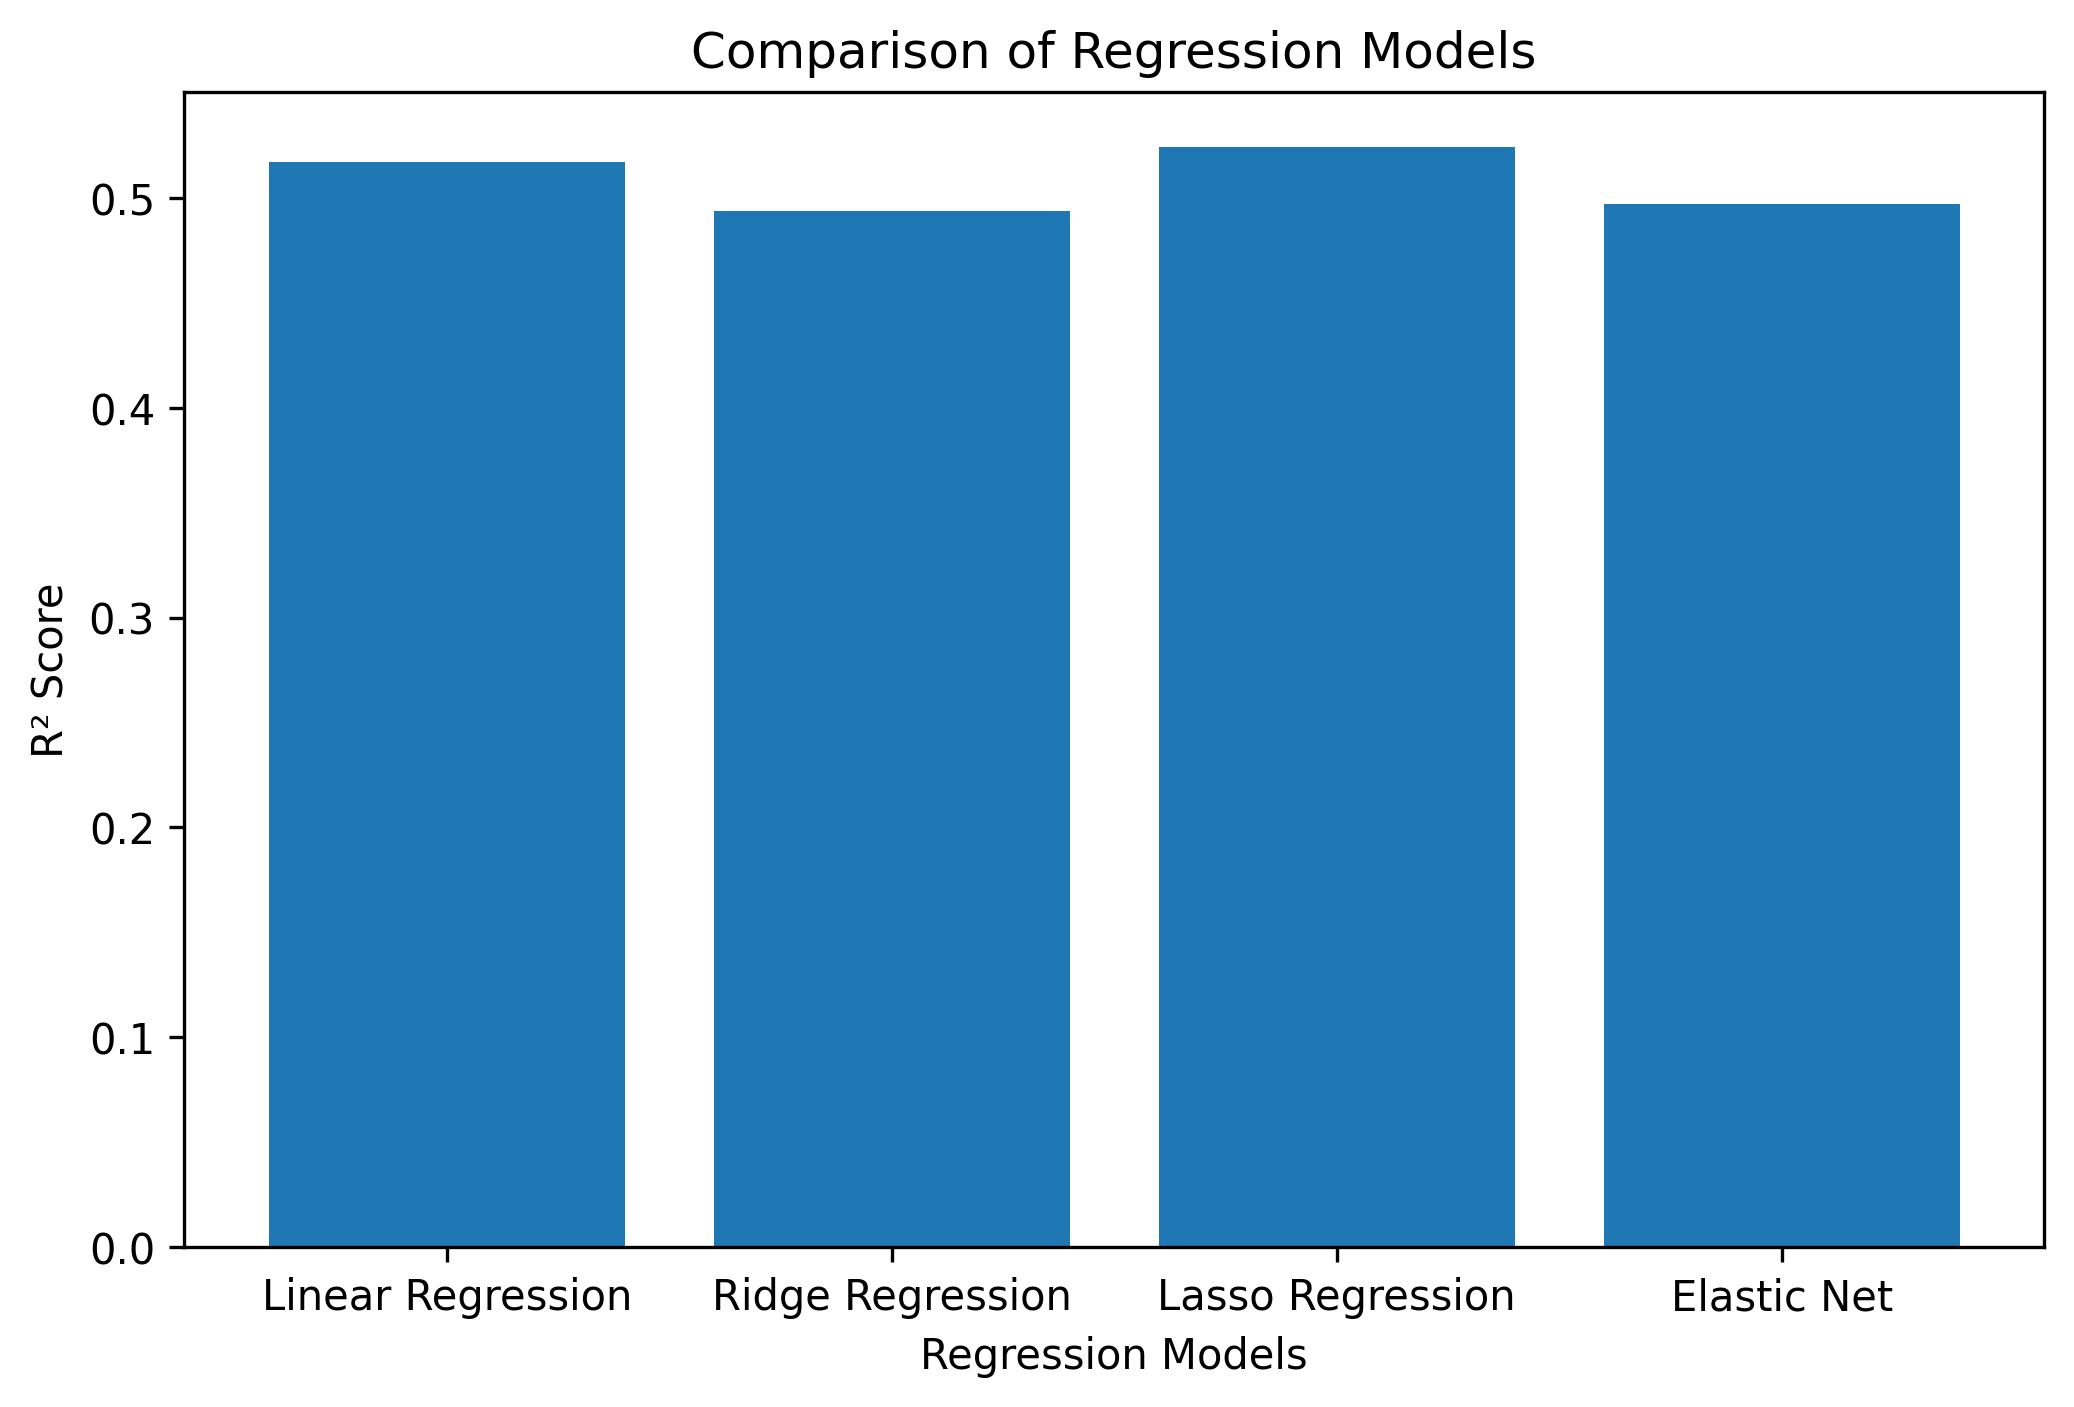
\includegraphics[width=0.75\linewidth]{model_comparison.png}
\caption{Comparison of Regression Models}
\end{figure}

\textbf{Inference:}
\begin{itemize}
\item Linear Regression achieved the highest R² score.
\item Lasso and Ridge Regression produced comparable performance.
\item Elastic Net showed slightly lower prediction accuracy.
\end{itemize}
%%%%%%%%%%%%%%%%%%%%%%%%%%%%%%%%%%%%%%%%%%%%%%%%%%%%%%%%%%%%%%%%%%%%%%
\section{Discussion}

Four regression models were implemented and compared for predicting loan amounts. Linear Regression achieved the best performance with the highest $R^2$ score and the lowest prediction error. Ridge and Lasso Regression produced similar results while reducing overfitting through regularization. Elastic Net Regression also performed well but showed slightly lower accuracy than the other models. Overall, Linear Regression was the most suitable model for this dataset.
%%%%%%%%%%%%%%%%%%%%%%%%%%%%%%%%%%%%%%%%%%%%%%%%%%%%%%%%%%%%%%%%%%%%%%
\section{Conclusion}

The Loan Amount Prediction dataset was successfully preprocessed by handling missing values, encoding categorical variables, and scaling the features. Linear Regression, Ridge Regression, Lasso Regression, and Elastic Net Regression were trained and evaluated using MAE, MSE, RMSE, and $R^2$ Score. Among all models, Linear Regression achieved the best performance. This experiment demonstrates the effectiveness of regression techniques for predicting loan amounts..

%%%%%%%%%%%%%%%%%%%%%%%%%%%%%%%%%%%%%%%%%%%%%%%%%%%%%%%%%%%%%%%%%%%%%%
\section{References}

\begin{enumerate}
    \item Gareth James et al., \textit{An Introduction to Statistical Learning}, Springer, 2021.
    \item Aurélien Géron, \textit{Hands-On Machine Learning with Scikit-Learn, Keras, and TensorFlow}, O'Reilly, 2022.
    \item Christopher M. Bishop, \textit{Pattern Recognition and Machine Learning}, Springer, 2006.
    \item \textit{Scikit-learn Documentation}: https://scikit-learn.org/
    
\end{enumerate}
\end{document}
